\documentclass[aspectratio=169]{beamer}

\newif\ifmore
\morefalse

\usepackage{inputenc}[utf8]
%\usepackage[polish]{babel}

%Lepiej tego nie zmieniaj, jak co to dodawaj pakiety
\usepackage{fancyhdr}
\usepackage{mdframed}
\usepackage{graphicx}
\usepackage{listings}
\usepackage{caption}
\usepackage{float}
\usepackage{tikz}
\usepackage{xcolor}
\usetikzlibrary{arrows}
\usepackage{hyperref}
\hypersetup{
    colorlinks=false,
    linkcolor=blue,
    filecolor=magenta,      
    urlcolor=cyan,
}
%\apptocmd{\frame}{}{\justifying}{} % Allow optional arguments after frame.

\urlstyle{same}
%Zmienne, zmień je!
\graphicspath{ {./ilustracje/} }
\title[How do video files work?]{How does digital video work?}
\author{Grzegorz Koperwas}
\date{\today}

%lokalizacja polska (odkomentuj jak piszesz po polsku)

%\usepackage{polski}
%\usepackage[polish]{babel} 
%\usepackage{indentfirst}
%\usepackage{icomma} 
\usetheme{Warsaw}

%\brokenpenalty=1000
%\clubpenalty=1000
%\widowpenalty=1000    

%nie odkometowuj wszystkiego, użyj mózgu
%\renewcommand\thechapter{\arabic{chapter}.}
%\renewcommand\thesection{\arabic{section}.}
%\renewcommand\thesubsection{\arabic{section}.\arabic{subsection}.}
%\renewcommand\thesubsubsection{\arabic{subsubsection}.}

%Makra

\newcommand{\obrazek}[2]{
\begin{figure}[h]
    \centering
    \includegraphics[scale=#1]{#2}
\end{figure}
}     
        

\newcommand{\twierdzonko}[1]{
    \begin{center}
    \begin{mdframed}
    #1
    \end{mdframed}          
    \end{center}
} 

\newcommand{\dwanajeden}[2]{
\ensuremath \left( \begin{array}{c}
    #1\\
    #2
\end{array} \right)
}  

\lstdefinestyle{json}{
    frame=trBL,
    numbers=left,
    basicstyle=\ttfamily\tiny,
    keywordstyle=\color{blue},
    morekeywords={ Metadata }
}


\begin{document}
\begin{frame}
    \titlepage
\end{frame}

\begin{frame}
    \tableofcontents
\end{frame}

\section{What are \texttt{.mkv}, \texttt{.mp4}, \texttt{.mov} etc.?}
\begin{frame}
    \frametitle{A "video file" is not just a video file}
    \begin{columns}
        \begin{column}{.5\textwidth}
            File formats such as \texttt{.mkv (matroska)} or \texttt{.mp4 (MPEG-4 part 14)} do not store video themselves.

            \pause
        \end{column}
        \begin{column}{.5\textwidth}
            \begin{block}{Definition}
                \textbf{Container format} - (sometimes called \emph{wrapper}) a file format that stores multiple data streams in one file.

                A common example would be a \texttt{ZIP} file, as it contains multiple files.
            \end{block}
        \end{column}
    \end{columns}
\end{frame}

%\begin{frame}
%    \frametitle{So what do they store?}
%    \framesubtitle{And how we can look at it?}
%    \begin{columns}
%        \begin{column}{.5\textwidth}
%            \texttt{FFmpeg} is a \emph{FOSS}
%            project that does multimedia.
%            \begin{description}
%                \item[ ffprobe ] - Displays information about multimedia (files, network or devices)
%
%                \item[ ffmpeg ] - Converts source (files, network or devices) to a format specified, can apply filters.
%            \end{description}
%        \end{column}
%        \begin{column}{.5\textwidth} 
%            
\includegraphics[width=\textwidth]{ffmpeg.png}
%        \end{column}   
%    \end{columns}
%\end{frame}

\begin{figure}
    \lstinputlisting[style=json]{anime.txt}
    \centering
\end{figure}

\section{What is a codec?}
\begin{frame}
    \frametitle{What is a codec?}
    \begin{columns}
        \begin{column}{ .5\textwidth }
            \textbf{Codec} is a software or hardware that encodes or decodes data, that is stored in a specified standard format. That data might be compressed, but does not need to be.

            \pause\vspace{.5cm}

            \textbf{Format} is a specification, that describes the way data will be stored.
        \end{column}
        \begin{column}{.5\textwidth}
            For example:
            \begin{description}
                \item[format: \texttt{h.264}] codec: \texttt{libx264}
                \item[format: \texttt{mp3}] codec: \texttt{libmp3lame}
            \end{description}
        \end{column}
    \end{columns}
\end{frame}

\begin{frame}
    \frametitle{What does effect picture quality?}
    \begin{description}
        \item[bitrate] - How much data is the stream allowed to take up in a unit of time, you can usually set it as a min/max value.
        \item[CRF] - Alternative to bitrate, what is the target quality, encoder will vary the bitrate accordingly.
        \item[patience] - Some encoders can do a better job if they are given more time, much more time.
        \item[pixel format]
    \end{description}
\end{frame}

\section{Pixel formats}

\begin{frame}
    \frametitle{What is a pixel format?}
    \begin{columns}
        \begin{column}{.5\textwidth}
            Pixel format is specified in part by bit depth (aka number of colors):

            \begin{figure}
                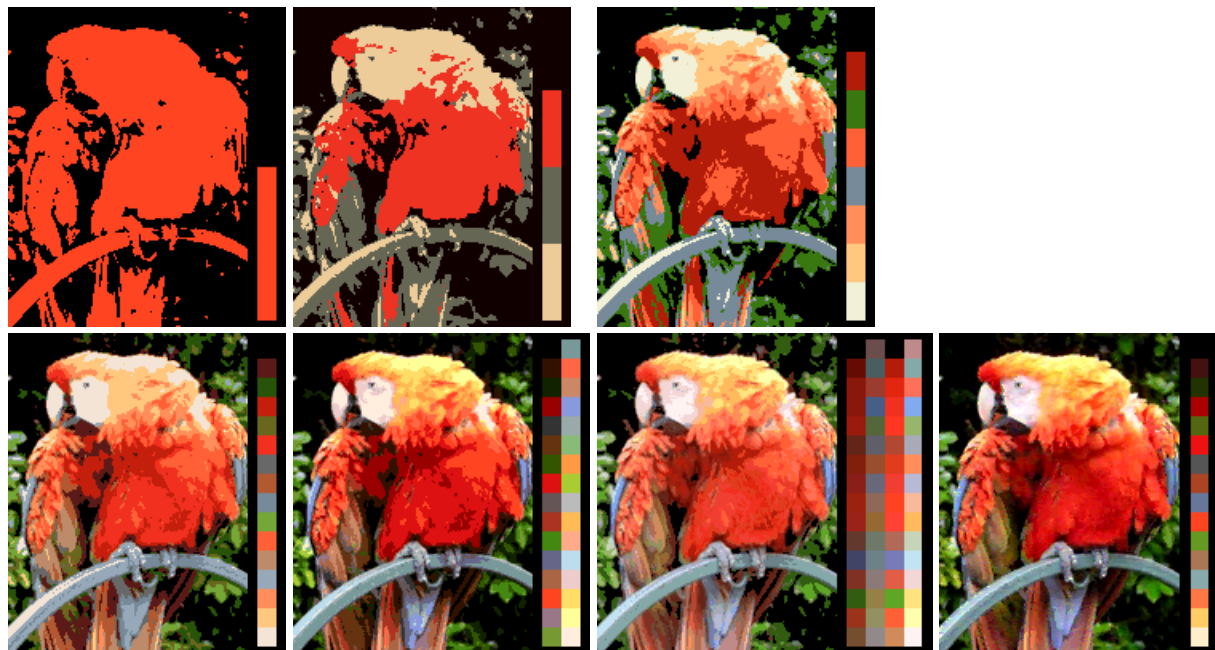
\includegraphics[width=\textwidth]{colors.png}
                \centering
            \end{figure}
            Most common bit depth is 24, also known as ``milions of colors''
        \end{column}
        \begin{column}{.5\textwidth}
            Pixel format also includes information about \emph{chroma subsampling}.
        \end{column}
    \end{columns}
\end{frame}

\begin{frame}
    \frametitle{What is chroma subsampling?}
    Instead of \textbf{RGB} we can use other formats such as \textbf{$YC_bC_r$}:
    \begin{description}
        \item[Y] - Luminance, or ``Black\&White''
        \item[$C_bC_r$] - Chroma, or ``Color''
    \end{description}
    \pause
    As humans are bad at perceiving color, but better at perceiving brightness, we can store $C_bC_r$ at a lower resolution.
    \pause
    \begin{columns}
        \begin{column}{.55\textwidth}
            \begin{figure}
                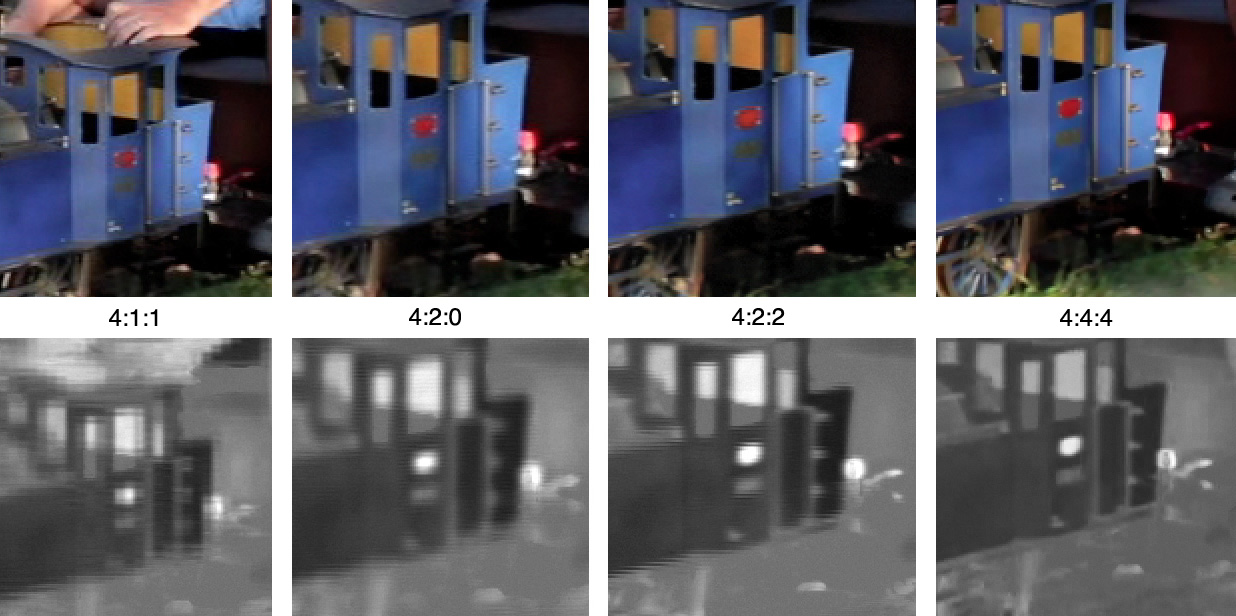
\includegraphics[width=\textwidth]{ycbcr.jpg}
                \centering
            \end{figure}
        \end{column}
    \end{columns}
\end{frame}

\begin{frame}
    \frametitle{The end!}
    Sources:
    \begin{itemize}
        \item Wikipedia articles
        \item FFmpeg wiki
        \item Technology Connections - ``Lines of Light: How Analog Television Works''
    \end{itemize}
\end{frame}
\end{document}
